\subsection{Airfoil Analysis}
The desired cruise conditions of Mach 0.775 and wing Reynolds number 4x$10^7$ for the aircraft fall within the transonic speed regime.  While this provides favorable conditions for the sizing analysis, the effects of wave drag increase as the aircraft approaches supersonic regime.  As shown in Figure \ref{fig:transonic} from Raymer\cite{raymer}, the effects of wave drag is observed to increase as Mach number increases.  Comparable aircraft combine use of supercritical airfoil and quarter chord sweep angles to delay the separated boundary layer due to shock.  Therefore, a selection of supercritical airfoils and wing sweep of no less than $32\degree$ is proposed to mitigate the increased effects of wave drag. \hl{re-add reference that was removed from fig 11 (see comment) to keep numbering correct}

\begin{figure}[!h]
    \centering
    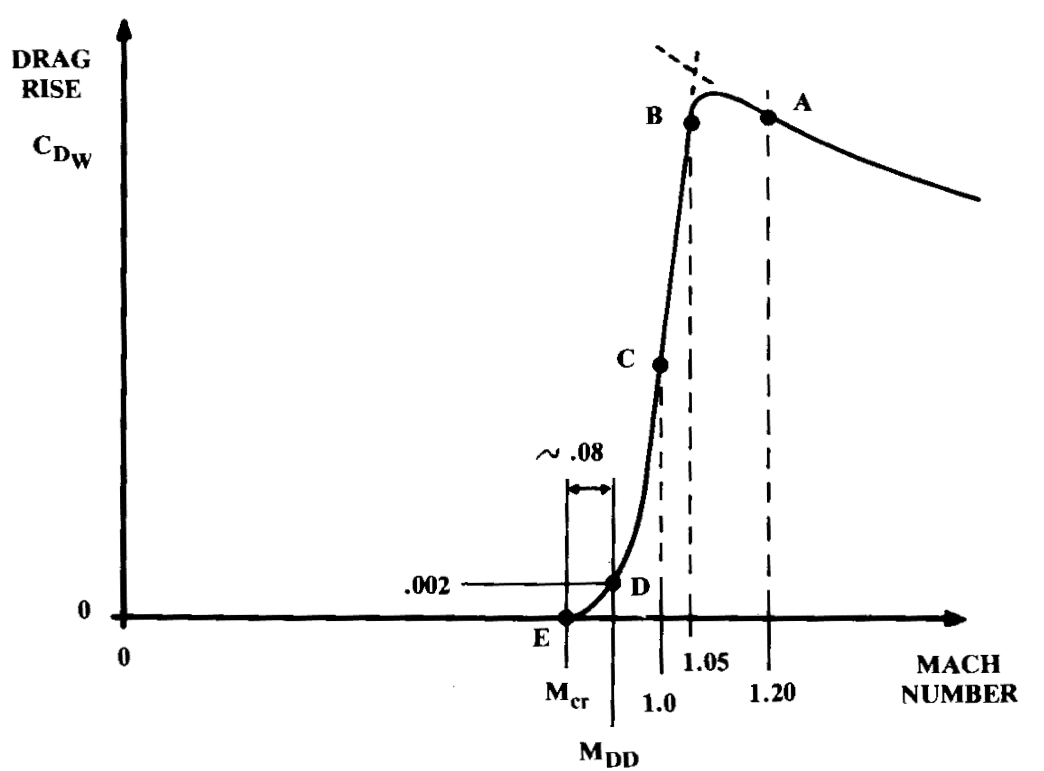
\includegraphics[width=0.65\textwidth]{Photos/wavedragduetotransonic.png}
    \caption{Wave Drag due to Transonic Airspeed}
    \label{fig:transonic}
\end{figure}

\subsubsection{Airfoil Trade Study}
A trade study is conducted comparing the fundamental characteristics between NACA 5-series airfoils and NASA supercritical airfoils.  Information learned in a NASA study \cite{supercritical} demonstrated the benefits of supercritical airfoils in delaying $M_{DD}$ such the wave drag is mitigated.  Consequently, several supercritical SC(2)-series airfoils, illustrated in Figures \ref{fig:0412airfoil} - \ref{fig:0712airfoil}, are initially selected and compared.  The supercritical airfoils are proposed due to their ability to delay the drag divergence mach number.  Using XFLR5 \cite{xflr5} incompressible flow analysis for take-off conditions, a simulation is processed to provide numerical data.  The results of some preliminary analyses through XFLR5 are listed below in Figure \ref{fig:airfoils}.  It is important to note these methods do not offer accurate analysis of the fluid behavior at transonic cruise conditions.  Rather, XLFR5 provides initial guidance for airfoil selection for take-off and landing segments.
\newpage

The airfoil cross section may be seen below in Figures \ref{fig:0412airfoil} - \ref{fig:0712airfoil} and the relevant information tabulated in Table \ref{tab:airfoils} and is generated with the coordinate values from UIUC Airfoil Coordinates Database \cite{selig} in XFLR5.

\begin{table}[!h]
    \centering
    \caption{Selected Airfoils}
    \begin{tabular}{|c|c|c|c|} \toprule
        \textbf{Airfoil Type} & \textbf{Figure} & \textbf{Max Thickness} & \textbf{Max Camber}\\ \hline \hline
        SC(2)-0412 & \ref{fig:0412airfoil} & $12\%$ at $37\%$ chord & $1.3\%$ at $83\%$ chord \\ \hline
        SC(2)-0714 & \ref{fig:0612airfoil} & $12\%$ at $37\%$ chord & $1.9\%$ at $81\%$ chord \\ \hline
        SC(2)-0612 & \ref{fig:0712airfoil} & $12\%$ at $37\%$ chord & $2.2\%$ at $81\%$ chord \\ \bottomrule
    \end{tabular}
    \label{tab:airfoils}
\end{table}

\begin{figure}[!h]
    \centering
    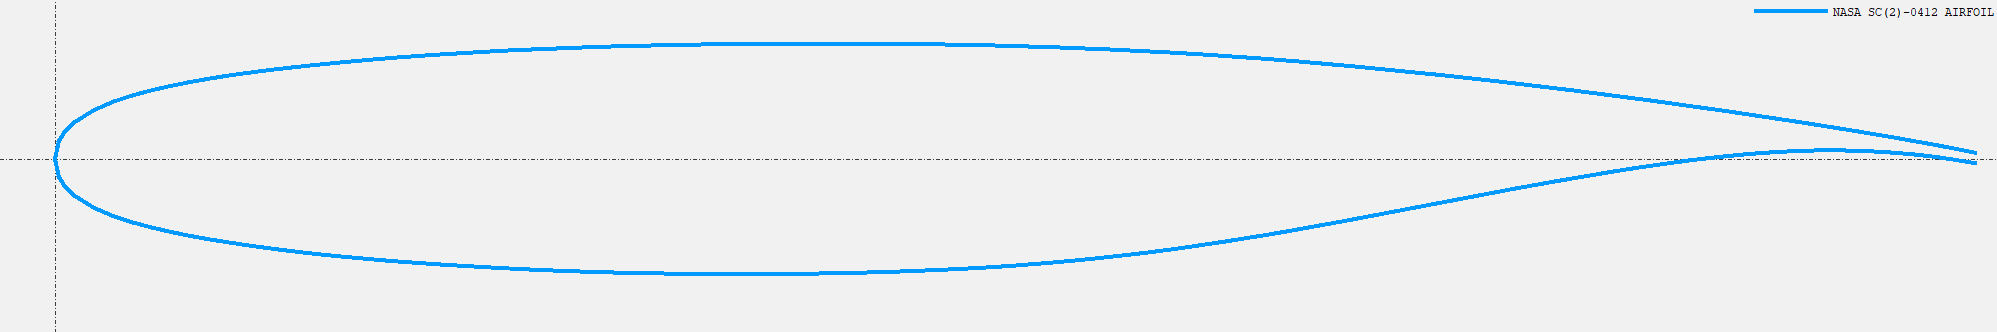
\includegraphics[width=\textwidth]{Photos/aero/sc0412.png}
    \caption{NASA SC(2)-0412 Airfoil Cross-Section}
    \label{fig:0412airfoil}
\end{figure}
\begin{figure}[!h]
    \centering
    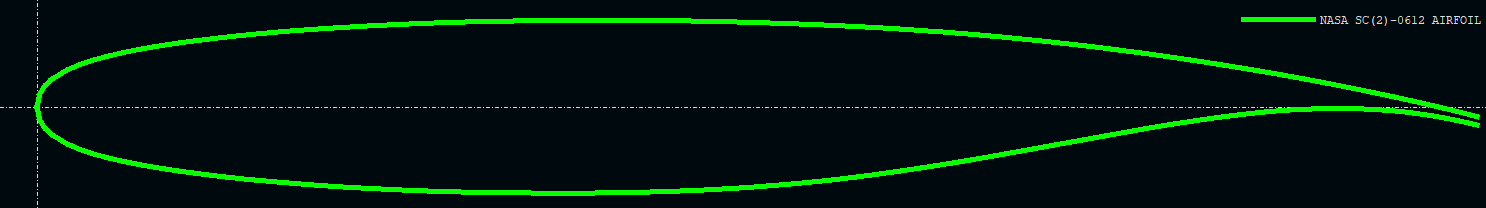
\includegraphics[width=\textwidth]{Photos/aero/sc0612.png}
    \caption{NASA SC(2)-0612 Airfoil Cross-Section}
    \label{fig:0612airfoil}
\end{figure}
\begin{figure}[!h]
    \centering
    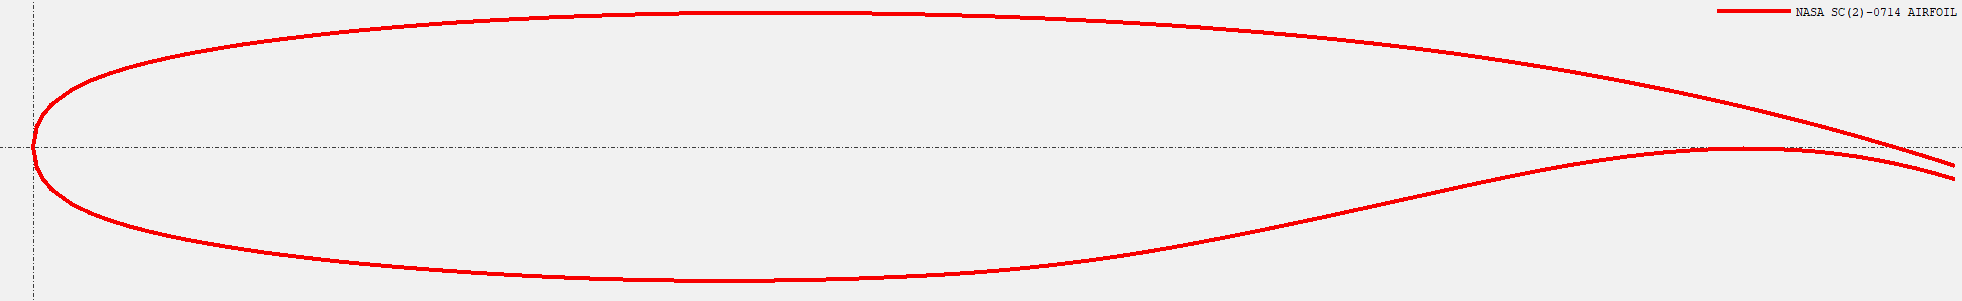
\includegraphics[width=\textwidth]{Photos/aero/sc0714.png}
    \caption{NASA SC(2)-0712 Airfoil Cross-Section}
    \label{fig:0712airfoil}
\end{figure}
\clearpage
\begin{figure}[!h]
    \centering
    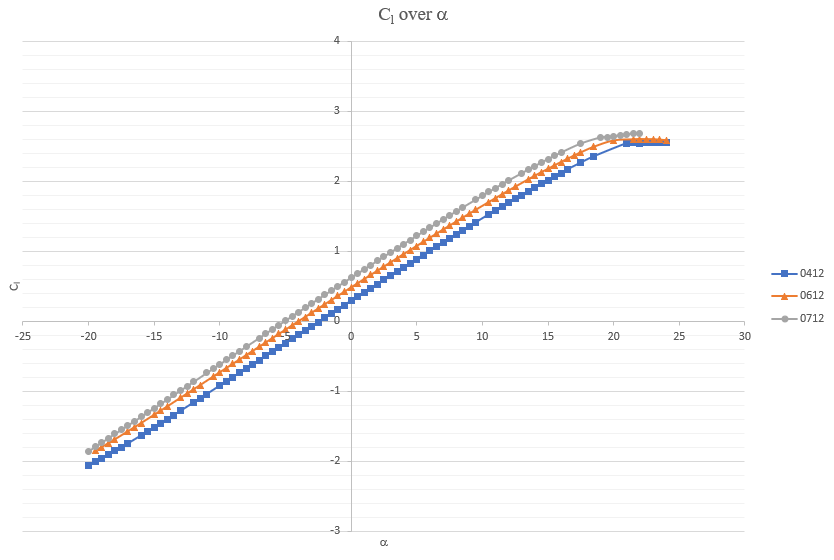
\includegraphics[width=\textwidth]{Photos/aero/AirfoilAnalysis.png}
    \caption{Airfoil $C_L$ vs $\alpha$ Comparison}
    \label{fig:airfoils}
\end{figure}

As shown above in the graphical analysis of the $C_l$ vs $\alpha$ polar, Figure \ref{fig:airfoils}, a favorable increase in lift coefficient results from SC(2)-0712.  Due to the mission requirement of serving as a high-capacity, medium-range aircraft, it is proposed to use the NASA SC(2)-0412 supercritical airfoil.  While the SC(2)-0714 airfoil presented favorable lift coefficients, the SC(2)-0412 resulted in a higher stall angle of attack with a minimal penalty difference of $\Delta C_l = -0.1392$.  The SC(2)-0412 airfoil is continuous for the entire span of its wing.  Aerodynamic twist is not introduced for fabrication efficiency and cost saving.  Later analyses in Section \ref{sec:highlift} observe the impacts of high lift devices such as Fowler Flaps and leading edge slats.


\newpage
\subsection{Wing Design}
Initial assumptions were made for the aspect ratio of the wing design based on comparable aircraft such as the Boeing 777-200 and Boeing 787.  Consequently, a range of aspect ratios, AR $ \in [8,12]$ was initially set.  A wing area of $5,000 \text{ ft}^2$ was recommended from the initial performance analysis.  More detailed contour analysis proved better range performance and weight saving with a wing reference area of $4,000 \text{ ft}^2$, as shown in Figure \ref{fig:contourf}.

\begin{figure}[!h]
    \centering
    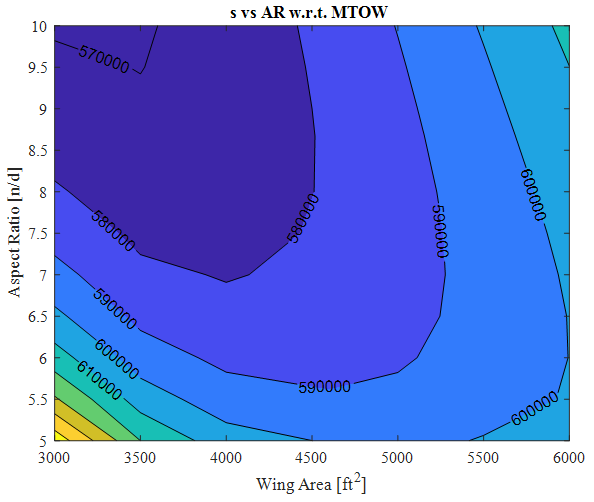
\includegraphics[width=0.85\textwidth]{Photos/aero/ARWingcontourf.png}
    \caption{Correlation among Wing area, Aspect Ratio, and Aircraft Maximum Take-off Weight}
    \label{fig:contourf}
\end{figure}

The modified wing dimensions are shown to the below in Table \ref{tab:wingsizing}.  The modified values provided a much more realistic wing span for the requirements.  Next steps involve generating the wing geometry in XFLR5 to determine aerodynamic characteristics.  The entire span of the wing uses the SC(2)-0412 airfoil with a dihedral angle of $2.5\degree$ and angle of incidence of $2.5 \degree$.  The angle of incidence improved the take-off and landing performance by increasing the coefficient of lift with minimal drag penalty.  Further studies into the effects of dihedral angle on the stability of the aircraft will be discussed in Section \ref{section: Stab and Control}.


\begin{figure}[!h]
    \centering
    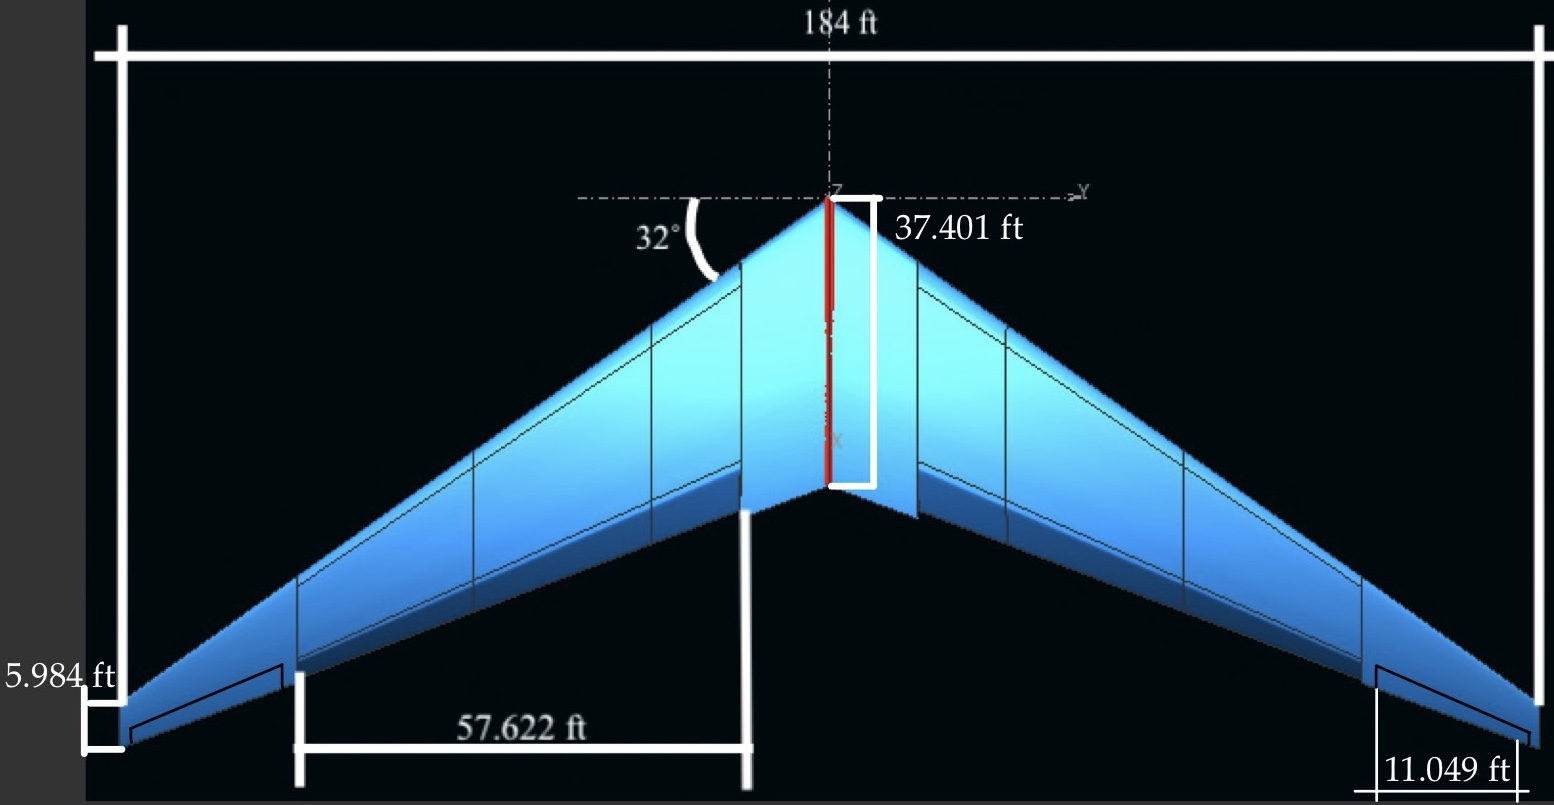
\includegraphics[width=0.95\textwidth]{Photos/aero/wing_flapped.png}
    \caption{Wing Dimension with Flaps and Slats}
    \label{fig:winged}
\end{figure}

\begin{table}[!h]
    \centering
    \caption{Wing Dimensions}
    \begin{tabular}{|c|c|c|c|} \toprule
        \multicolumn{4}{c}{\textbf{\textcolor{cobalt}{Main Wing}}} \\ \midrule
        \textbf{Description} & \textbf{Initial \#} & \textbf{Finalized \#} & \textbf{Units} \\ \hline \hline
        AR & 9.0 & 8.5 & $\sim$ \\ \hline
        b (\textit{span}) & 212 & 184 & ft \\ \hline 
        $s_{\text{wing}}$ (\textit{area}) & 5,000 & 4,000 & ft$^2$ \\ \hline
        c/4 Sweep & 30 & $32$ & degree \\ \hline
        $\alpha_i$ & 0 & $2.5$ & degree \\ \hline
        $+\Gamma$ (\textit{dihedral}) & 0 & $2.5$ & degree \\ \hline
        $\lambda$ & 0.18 & 0.16 & $\sim$ \\ \hline
        Chord Root & 479.39 & 452.72 & in \\ \hline
        Chord Tip & 86.29 & 67.91 & in \\ \hline   
        Mean Aerodynamic Chord & 328.37 & 307.72 & in \\ \bottomrule
    \end{tabular}
    \label{tab:wingsizing}
\end{table}
\clearpage

\subsection{High-Lift Systems}\label{sec:highlift}
High-lift devices are implemented on SAM Mk I to improve aircraft stability during take-off and landing segments of the mission profile.  Leading edge slats and trailing edge Fowler flaps are included on the wing.  The analysis for high-lift devices included five different configurations, as tabulated below in Table \ref{tab:highlyfttest}.  Due to XFLR5's incompressible and low Reynolds number limitations, take-off condition is assumed for $V_{TR} = 281.2$ ft/s.

\begin{table}[!h]
    \centering
    \caption{Analysis of High-Lifting Devices}
    \begin{tabular}{|p{1in}|p{1in}|p{0.5\textwidth}|}\toprule
        \textbf{Configuration} & \textbf{Graphical Color} & \textbf{Description}\\\hline \hline
        Flaps 0 & Cyan & $\delta_F=0\degree$ and no slats \\ \hline
        Flaps 1 & Purple & $\delta_F = 10\degree$ and full slats \\ \hline
        Flaps 2 & Red & $\delta_F = 20\degree$ and full slats \\\hline
        Flaps 3 & Orange & $\delta_F = 30\degree$ and full slats \\\hline
        Slat Test & Green & $\delta_F = 30\degree$ with No Slats \\ \bottomrule
    \end{tabular}
    \label{tab:highlyfttest}
\end{table}

\begin{figure}[!h]
    \centering
    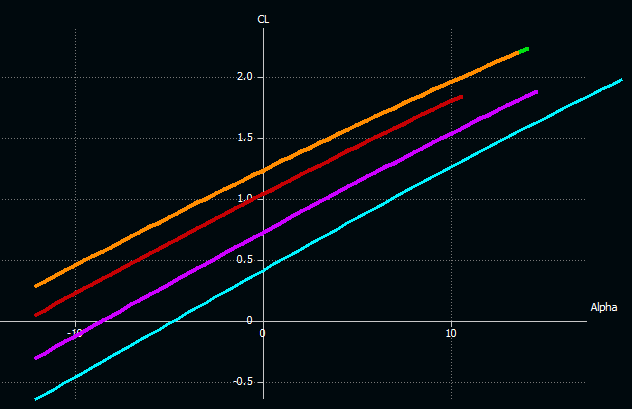
\includegraphics[width=0.70\textwidth]{Photos/aero/CL_o_alpha.png}
    \caption{$C_L$ vs. $\alpha$ for varying $\delta_F$}
    \label{fig:clalphahigh}
\end{figure}
According to Figure \ref{fig:clalphahigh}, Flap setting three provides optimal lift coefficient and is recommended for a full flaps take-off configuration.  Further analysis will determine whether Flaps 3 is also an appropriate setting for landing.  Figure \ref{fig:clcdalphahigh} displays the significant increase in drag with an increase of flap deflection.  As a result, Flap setting zero is recommended for cruise to optimize aerodynamic performance.  Additionally, the studies show smoother and steadier polars for flap conditions combined with slats.  Therefore, a recommendation of combining slats and flaps is made for SAM Mk I.

\begin{figure}[!h]
    \centering
    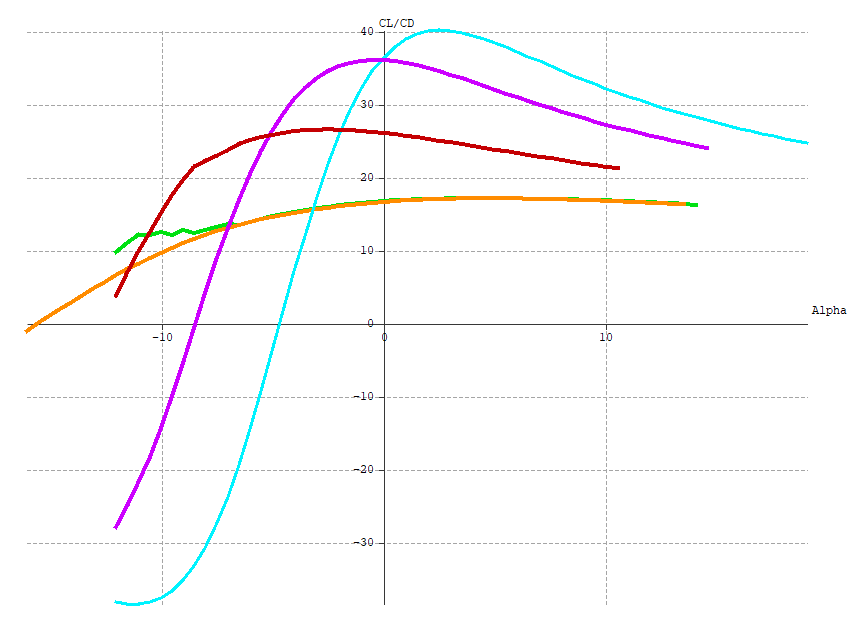
\includegraphics[width=0.65\textwidth]{Photos/aero/CL_CD_o_alpha.png}
    \caption{$\frac{C_L}{C_D}$ vs $\alpha$ for varying $\delta_F$}
    \label{fig:clcdalphahigh}
\end{figure}

\begin{figure}[!h]
    \centering
    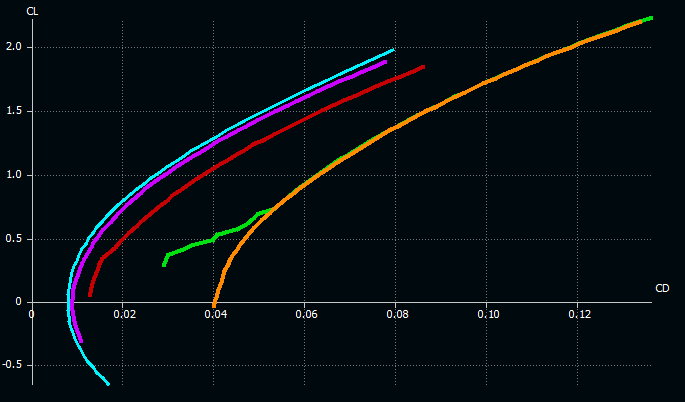
\includegraphics[width=0.65\textwidth]{Photos/aero/CL_o_CD.png}
    \caption{$C_L$ vs $C_D$ for varying $\delta_F$}
    \label{fig:clcdhigh}
\end{figure}

\begin{figure}[!h]
    \centering
    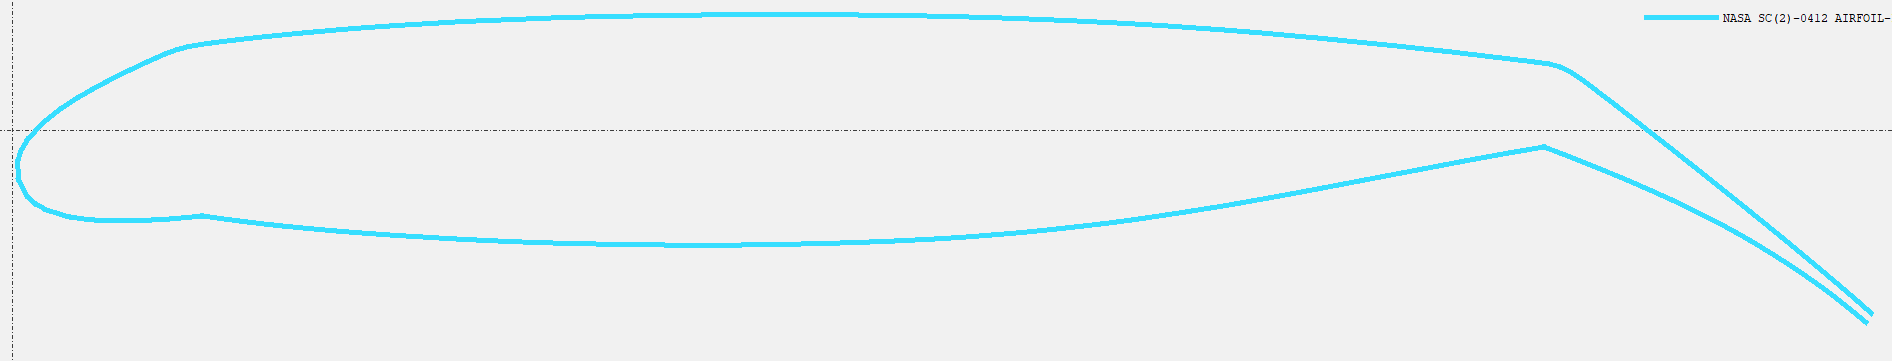
\includegraphics[width=\textwidth]{Photos/aero/sc0412flapped.png}
    \caption{SC(2)-0412 Airfoil with $\delta_F = 30\degree$ and slats}
    \label{fig:highlift}
\end{figure}

\clearpage
\subsection{Drag Buildup}
The Drag for SAM Mk. I is built up part-by-part by separating the fuselage, wings, empennage, and other protuberances and calculating the following seven key forms of drag, shown in Equation \ref{eqn:drag_general} from Raymer \cite{raymer}:
\begin{equation}\label{eqn:drag_general}
    C_D = C_{D,0} + C_{D,i} + C_{D,W_{NL}} + C_{D,W_{L}} + C_{D_{EXCR}} + \Delta C_{D_{Re}} + C_{D,trim}
\end{equation}


% \subsubsection{Take-Off Drag}


% \subsubsection{Cruise Drag}
To properly predict and quantify the wave drag for aerodynamic analysis on the airfoil and wing design, two methods are tested: \textit{Method B} from Vargas et al. \cite{vargas} and \textit{Delta Method} from Feagin \cite{deltaMethod}.  The Delta method relies on a combination of graphical comparison offsetting the McDevitt method \cite{mcdevitt} by adding the Torenbeek method \cite{torenbeek} to account for the transonic flow characteristics.  Through a graphical approach and MATLAB computed analysis, the Cruise Drag buildup is displayed in Table \ref{tab:dragbuildup}.

\begin{table}[!h]
    \centering
    \caption{Tabulated Drag Buildup}
    \begin{tabular}{|p{0.75in}|p{0.75in}|p{0.75in}|p{0.75in}|p{0.75in}|p{0.75in}|}\toprule
        \textbf{Description} & \textbf{Wing} & \textbf{Vertical \newline Stabilizer} & \textbf{Horizontal \newline Stabilizer} & \textbf{Fuselage} & \textbf{Nacelle}  \\ \midrule \hline
        $S_{wet} (ft^2)$ & 8,095 & 1,012 & 2024 & 11,384 & 1,194 \\ \hline
        Reynolds Number & $4.77x10^7$ & $3.68x10^7$ & $3.01x10^7$ & $4.36 x 10^8$ & $5.46 x 10^7$ \\ \hline
        $C_{f}$ & $2.306 x 10^{-3}$ & $2.388 x 10^{-3}$ & $2.455 x 10^{-3}$ & $1.596 x 10^{-3}$ & $2.163 x 10^{-3}$ \\ \hline
        $FF$ & $1.570$ & $1.3500$ & $1.3500$ & $1.046$ & $1.184$ \\ \hline
        \textbf{$(C_{D_{0}})_{cruise}$} & $6.196 x 10^{-3}$ & $7.700 x 10^{-4}$ & $1.583 x 10^{-3}$ & $4.486 x 10^{-3}$ & $7.217x10^{-4}$ \\ \midrule
        \textbf{$C_{D,W}$} & $3.214 x 10^{-3}$ & $\sim$ & $\sim$ & 0 & $\sim$ \\ \hline
        
    \end{tabular}
    \label{tab:dragbuildup}
\end{table}

In calculating the total parasitic drag, $C_{D_{0}}$ of SAM Mk I, an additional two to five percent increase in drag accounts for the leakage and protuberance drag. \cite{raymer}  Using a part-by-part analysis and including the Delta method to account for wave drag, the estimated total coefficient of drag during cruise is $3.211 x 10^{-2}$.

\subsection{Justification for Adding a Winglet}



%%% Rubbish Bin of Joshua's failure/sadness:

% \subsection{Future Progress} lol I was about to highlite future progress for removal I gotcha lol :P
% Several key topics are under active investigation to improve the aircraft performance. The following will be further investigated for the Preliminary Design Report:
% \begin{itemize}
%     \item Confirm Drag Coefficients for take-off and landing analysis
%     \item Investigate use of Flaperons for cruise roll stability
%     \item CFD analysis of complete wing and body system
% \end{itemize}


% \textcolor{red}{
% \begin{itemize}
%     \item Discuss airfoil selection, including reasoning, lift curves, drag polar.
%     \begin{itemize}
%         \item Selection should not solely be from using XFOIL! \checkmark
%         \item Airfoil selection should encompass multiple methods \checkmark
%     \end{itemize}
%     \item Discuss wing design, including reasoning, geometry, and CAD drawings with dimensions \checkmark
%     \begin{itemize}
%         \item Label diagram and tabulate important parameters. \checkmark
%     \end{itemize}
%     \item CAD is expected for major drawings \checkmark (thx chris)
%     \item Discuss high-lift system, including reasoning, geometry, and CAD drawings with dimensions \checkmark
%     \item Discuss drag buildup (tabulated), including cruise, takeoff, and landing \checkmark
%     \begin{itemize}
%         \item Describe your methods and include significant contributions \checkmark
%     \end{itemize}
%     \item Discuss aircraft lift curves and drag polars, including cruise, takeoff, and landing. \checkmark
%     \begin{itemize}
%         \item Identify key mission points on these plots. \checkmark
%         \item Describe methods and limitations. \checkmark
%     \end{itemize}
%     \item Summarize key aircraft information (tabulated) at cruise, takeoff, and landing (e.g. angle of attack, lift coefficient, drag coefficient).
%     \item Include at least two trade studies that use quantitative analysis to support design decisions made.
%     \begin{itemize}
%         \item One should be airfoil selection
%         \item Describe system-level tradeoffs (if any)
%     \end{itemize}
%     \item Discuss parachute sizing if required.
%     \item Discuss future work.
%     \item \hl{Important aerodynamic characteristics and aerodynamic performance for key mission segments and requirements AERO or PERF}
% \end{itemize}}